\documentclass[conference]{IEEEtran}

\usepackage[utf8]{inputenc}
\usepackage[T1]{fontenc}
\usepackage[spanish, es-nodecimaldot]{babel}

\usepackage{amsmath}
\usepackage{amssymb}
\usepackage{array}
\usepackage{booktabs}
\usepackage{multirow}

\usepackage{graphicx}
\graphicspath{{figures/}}

\usepackage{url}
\usepackage{cite}

\spanishdecimal{.}

\begin{document}

\title{Tipologías de Patrón Productivo Agrícola en el Perú: un Modelo de \textit{Clustering} Independiente de la Geografía (2020--2025)}

\author{
\IEEEauthorblockN{Johao Mendoza, Joyssie Rivas, Thiago Ormeño}
\IEEEauthorblockA{\textit{Departamento de Ingeniería} \\
\textit{Universidad del Pacífico} \\
Lima, Perú \\
\{jr.mendozaf@alum.up.edu.pe, ja.rivasr@alum.up.edu.pe, tc.ormenof@alum.up.edu.pe\}}
}

\maketitle

\begin{abstract}
Este trabajo propone un modelo de \textit{clustering} no supervisado para tipificar cultivos agrícolas peruanos según su \emph{patrón productivo}, de forma independiente de su ubicación geográfica. Integrando producción mensual del MIDAGRI (2020--2025) y variables climáticas de NASA POWER en seis regiones bajo un enfoque multi-distrito por piso ecológico, se construyeron 33 perfiles región--cultivo. Se demuestra primero que el \textit{clustering} ingenuo sobre \textit{features} agroclimáticas reproduce la geografía (Índice de Rand Ajustado, ARI, $=0.59$ con la región) en lugar de tipificar cultivos, debido a la degeneración de las variables climáticas constantes por distrito. Como solución, el modelo propuesto describe cada cultivo mediante un vector de estacionalidad mensual (12 fracciones de producción anual), su escala logarítmica, concentración del mes pico y amplitud de cosecha, reduciendo el clima a dos componentes principales secundarios. El modelo KMeans resultante ($K=6$, Silhouette 0.30) alcanza un ARI de solo 0.06 con la región, evidenciando que el agrupamiento responde al comportamiento productivo y no a la geografía. Las seis tipologías --- permanente, mono-pico de otoño, concentrada de invierno, entre otras --- agrupan cultivos de regiones distintas que comparten calendario. El modelo ofrece una caracterización agronómicamente interpretable y reproducible, útil para planificación de cosechas y gestión de riesgo estacional.
\end{abstract}

\begin{IEEEkeywords}
Clustering, KMeans, estacionalidad, patrón productivo, agricultura, NASA POWER, MIDAGRI, CRISP-DM, Índice de Rand Ajustado
\end{IEEEkeywords}

\section{Introducción}
La agricultura representa el 4.8\% del PBI peruano en 2025 \cite{bcrp2025} y sus agroexportaciones casi se duplicaron entre 2020 y 2025 \cite{adex2026}. Caracterizar los cultivos según su comportamiento productivo --- cuándo cosechan, qué tan concentrada es su producción, qué escala alcanzan --- es relevante para la planificación de cosechas, la logística agroexportadora y la gestión del riesgo climático estacional.

El \textit{clustering} no supervisado es la herramienta natural para construir tales tipologías. Sin embargo, su aplicación al dominio agroclimático presenta un riesgo metodológico poco discutido: cuando los perfiles de cultivo se describen con variables climáticas y estas son constantes dentro de cada zona geográfica, el agrupamiento tiende a reproducir la geografía en lugar de capturar estructura productiva. El presente trabajo (i) diagnostica formalmente este sesgo mediante el Índice de Rand Ajustado, y (ii) propone un modelo de \textit{clustering} centrado en la estacionalidad productiva que se independiza de la geografía.

El objetivo es construir y validar un modelo de tipologías de patrón productivo para los cultivos dominantes de seis regiones peruanas (Ica, Junín, La Libertad, Piura, Puno y San Martín), bajo la metodología CRISP-DM \cite{inia2019, chapman2000}.

\section{Estado del Arte}
El uso de CRISP-DM y minería de datos en agricultura ha crecido recientemente \cite{chapapria2024, canchano2024}, con foco mayoritario en tareas predictivas de rendimiento o precios. Los trabajos de zonificación agroecológica \cite{midagri2025, una2023} reconocen la importancia del piso ecológico, pero suelen operar con agregados anuales o un único punto climático por región. En el plano del \textit{clustering}, la literatura agroclimática rara vez audita si la partición obtenida captura información productiva o si simplemente refleja la estructura espacial de los datos. Métricas internas como el coeficiente de Silhouette miden cohesión y separación, pero no distinguen una tipología agronómica genuina de una reproducción trivial de la geografía. Este trabajo cubre ese vacío empleando el Índice de Rand Ajustado frente a la región como diagnóstico explícito de validez.

\section{Metodología}

\subsection{Datos y enfoque multi-distrito}
Se integraron dos fuentes públicas bajo CRISP-DM: la hoja \texttt{c-18} del MIDAGRI \cite{midagrihist}, con producción acumulada por región, mes y cultivo (2020--2025), y variables climáticas de NASA POWER \cite{nasa2025}. La producción mensual se recuperó por diferenciación de acumulados, $Prod_m = Acum_m - Acum_{m-1}$, con manejo explícito de tres meses faltantes y de valores anómalos como NaN. Dada la heterogeneidad ecológica de las regiones peruanas, se muestrearon 14 distritos representativos por piso ecológico, evitando el sesgo de un único punto climático regional. Tras filtrar por Pareto-80 (cultivos que acumulan el 80\% de la producción regional), se obtuvieron 33 perfiles región--cultivo sobre 2{,}376 observaciones cultivo--mes.

\subsection{Diagnóstico del sesgo geográfico}
Como punto de partida se replicó el enfoque convencional: agrupar los 33 perfiles descritos por media y desviación de cinco variables climáticas más tres indicadores de producción. Para auditar la naturaleza de la partición se calculó el Índice de Rand Ajustado (ARI) entre las etiquetas de cluster y la región administrativa. Un ARI cercano a 1 indica que el modelo reproduce la geografía; cercano a 0, que captura estructura independiente de ella.

El diagnóstico es contundente: el modelo convencional ($K=6$, Silhouette 0.514) obtiene ARI $=0.59$ con la región, y eliminar las variables de producción altera la partición en menos del 20\% de los casos. La razón es estructural: como el clima es constante por distrito, las 10 \textit{features} climáticas solo toman 11 valores distintos y dominan numéricamente a las 3 productivas. El Silhouette elevado premia esta redundancia espacial. \emph{El modelo convencional no tipifica cultivos: reproduce regiones.} Esto motiva el modelo propuesto.

\subsection{Modelo propuesto: perfiles de patrón productivo}
Para que el cultivo determine el agrupamiento, cada perfil región--cultivo se describe con \textit{features} centradas en su comportamiento productivo y no en su clima:

\begin{itemize}
    \item \textbf{Estacionalidad (12 \textit{features}):} producción mensual sumada 2020--2025 y normalizada por el total anual, $f_m = \sum_y Prod_{m,y} / \sum_{m,y} Prod_{m,y}$, que describe la \emph{forma} del calendario productivo con independencia de la escala.
    \item \textbf{Escala:} $\log(1+\text{producción total})$, que comprime el rango de cinco órdenes de magnitud y neutraliza el \textit{outlier} de la caña de Virú (28\,M\,tn).
    \item \textbf{Concentración:} fracción del mes pico (1 = toda la producción en un mes).
    \item \textbf{Amplitud:} número de meses con cosecha y coeficiente de variación mensual.
    \item \textbf{Clima (2 \textit{features}):} dos componentes principales del clima del distrito, incluidas con peso reducido para que no dominen.
\end{itemize}

Las 18 \textit{features} se estandarizaron por $z$-score. Se aplicó KMeans con selección de $K$ por consenso entre Silhouette y Davies--Bouldin ($K=2,\dots,8$), validando la estructura con \textit{clustering} jerárquico de Ward y una proyección PCA.

\section{Resultados}

\subsection{Motivación empírica: concentración y estacionalidad}
La producción agregada se concentra fuertemente en pocas unidades región--piso (Fig.~\ref{fig:prod_unidad}), abarcando dos órdenes de magnitud entre la mayor (La Libertad--Costa, 36.8\,M\,tn) y la menor (Cascas--Yunga, 0.36\,M\,tn). Esta dispersión justifica la transformación logarítmica de la escala. A su vez, el patrón estacional (Fig.~\ref{fig:estacional}) muestra calendarios productivos muy distintos: la puna de Puno concentra su producción en abril--mayo, mientras que las costas de Ica y La Libertad producen de forma casi uniforme todo el año. Es precisamente esta forma del calendario --- y no el clima del lugar --- la que el modelo propuesto busca capturar.

\begin{figure}[h]
    \centering
    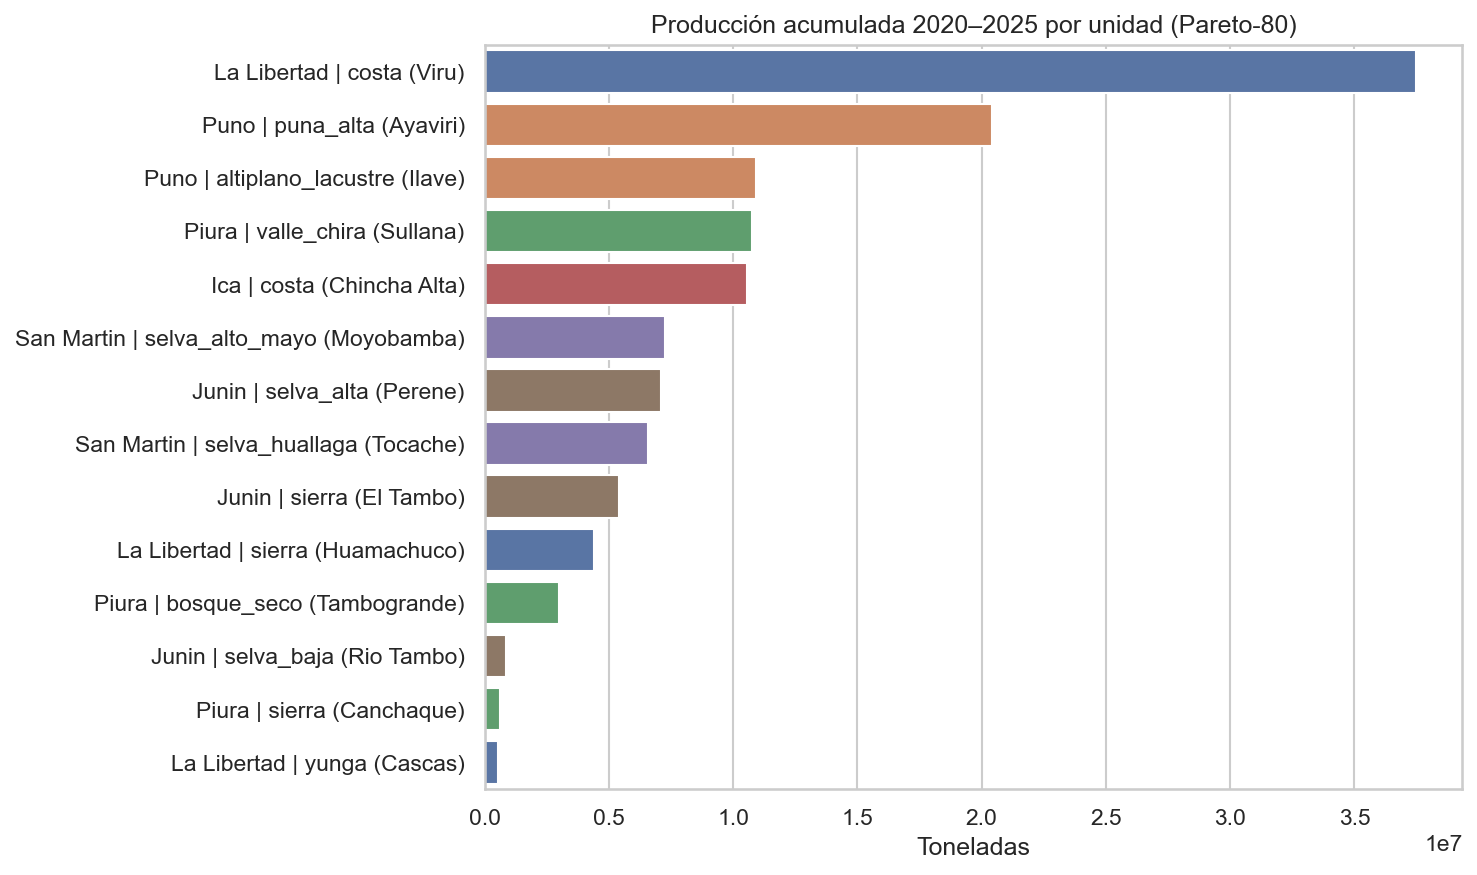
\includegraphics[width=0.46\textwidth]{eda_regional_volumen_unidad.png}
    \caption{Producción acumulada 2020--2025 por unidad región--piso. El rango de cinco órdenes de magnitud motiva la escala logarítmica.}
    \label{fig:prod_unidad}
\end{figure}

\begin{figure}[h]
    \centering
    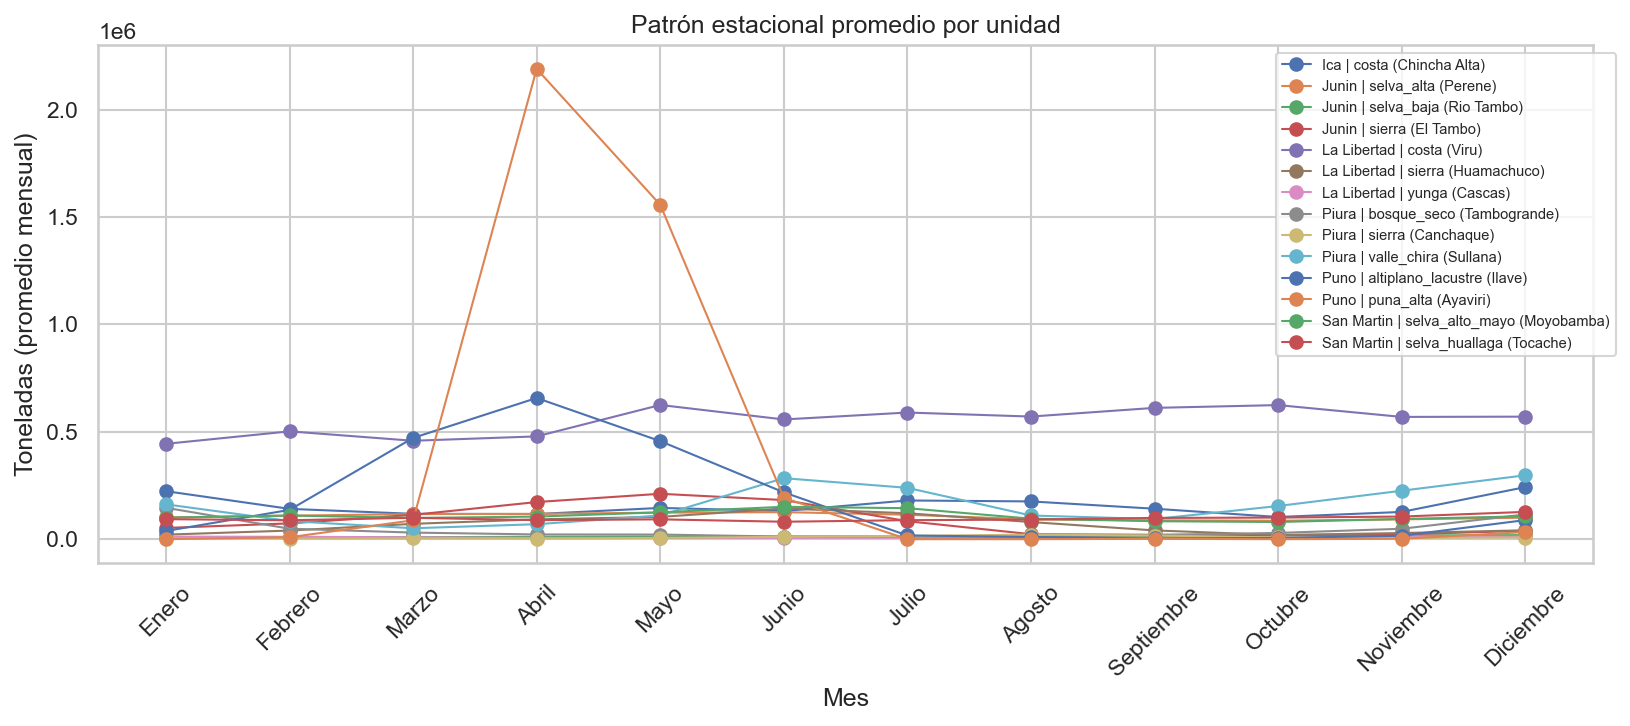
\includegraphics[width=0.48\textwidth]{eda_regional_patron_estacional.png}
    \caption{Patrón estacional promedio por unidad. Los calendarios productivos contrastan: la puna de Puno concentra en abril--mayo; las costas son uniformes.}
    \label{fig:estacional}
\end{figure}

Las correlaciones clima--cultivo (Fig.~\ref{fig:corr}) confirman que el clima por sí solo no individualiza bien a los cultivos de un mismo piso, ya que comparten el mismo forzamiento climático; el patrón productivo aporta la información discriminante que falta.

\begin{figure}[h]
    \centering
    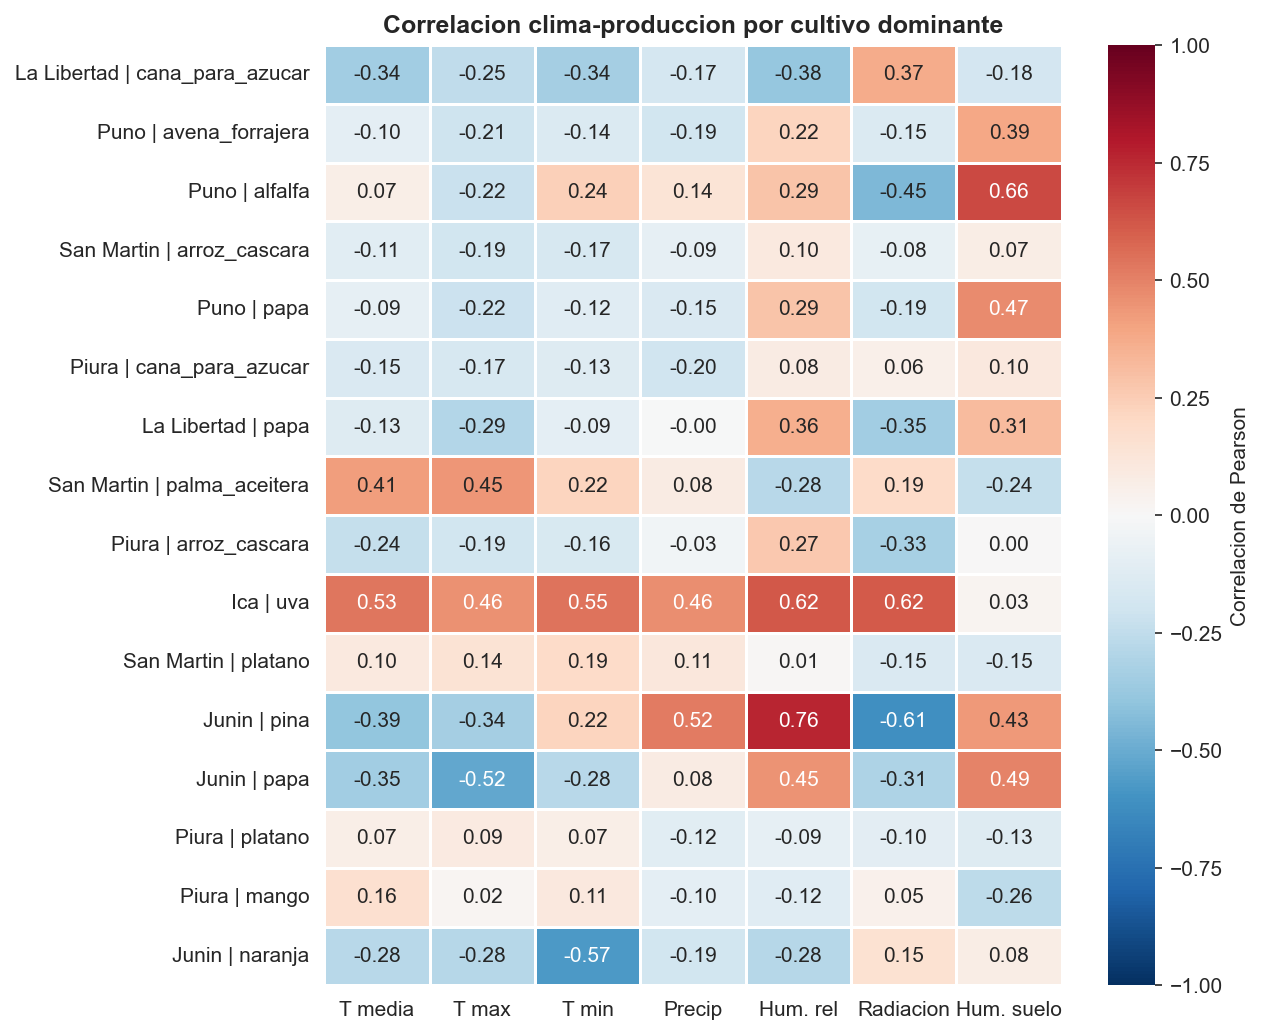
\includegraphics[width=0.48\textwidth]{corr_clima_cultivo.png}
    \caption{Correlación clima--producción por cultivo dominante. Cultivos del mismo piso comparten forzamiento climático, por lo que el clima discrimina poco entre ellos.}
    \label{fig:corr}
\end{figure}

\subsection{Tipologías de patrón productivo}
El modelo propuesto selecciona $K=6$ tipologías (Silhouette 0.30, Davies--Bouldin 0.90). El mapa de calor de estacionalidad por cluster (Fig.~\ref{fig:heatmap_b}) es el resultado central y permite nombrar cada tipología:

\begin{itemize}
    \item \textbf{Permanente / plano:} producción uniforme ($\approx0.08$--$0.11$ por mes); reúne espárrago de Ica, caña de La Libertad y Piura, palma y plátano de selva.
    \item \textbf{Concentrada de otoño:} pico en abril--mayo (fracción 0.52 en abril); forrajeras y papa del altiplano de Puno.
    \item \textbf{Concentrada de invierno:} pico en agosto (0.45); papa de Ica.
    \item \textbf{Bimodal de verano:} picos en enero y diciembre; tomate y uva de costa, mango de Piura.
    \item \textbf{Pico de otoño tardío} y \textbf{pico de mayo:} grupos intermedios con cosecha desplazada.
\end{itemize}

\begin{figure}[h]
    \centering
    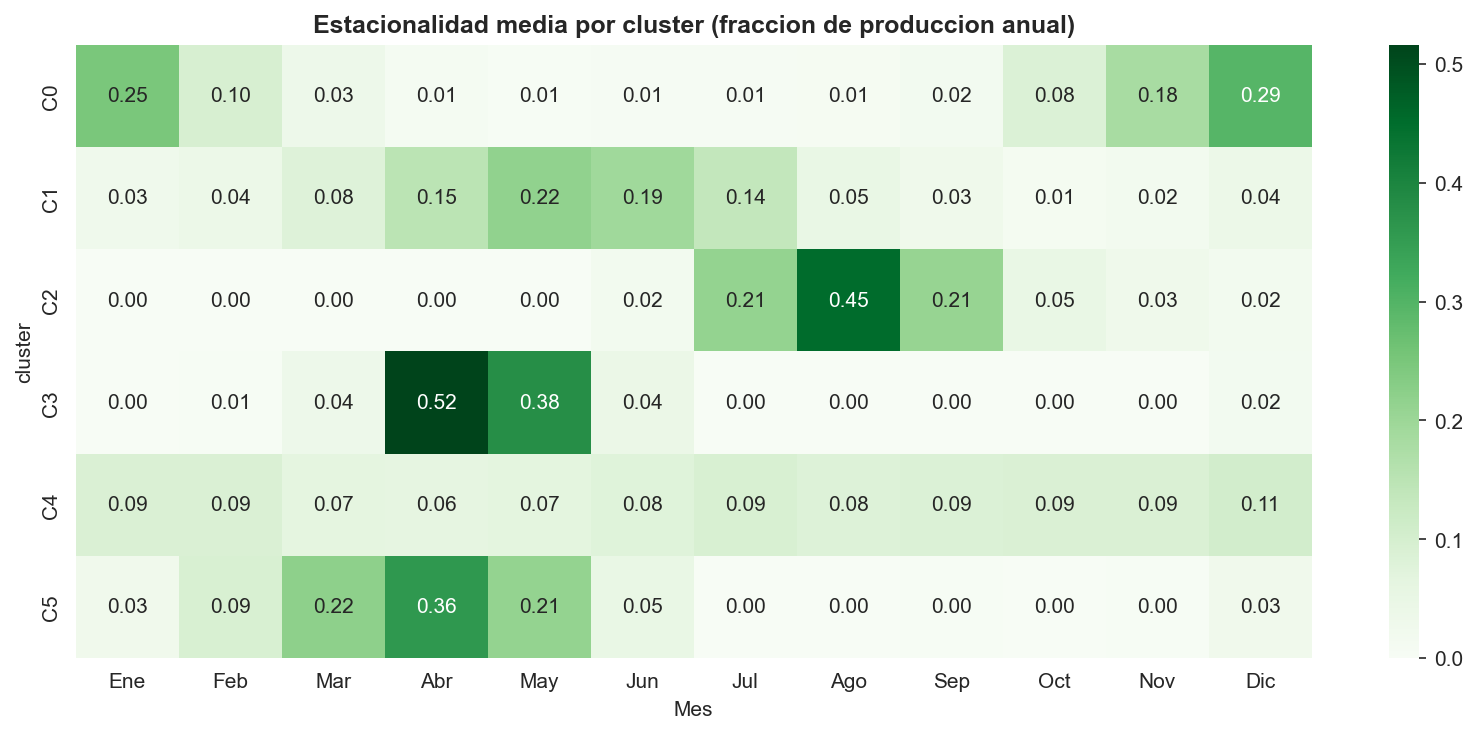
\includegraphics[width=0.48\textwidth]{06b_heatmap_estacionalidad.png}
    \caption{Estacionalidad media por cluster (fracción de producción anual por mes). Cada fila es una tipología de calendario productivo; resultado central del modelo.}
    \label{fig:heatmap_b}
\end{figure}

El dendrograma de Ward (Fig.~\ref{fig:dendro_b}) valida la estructura jerárquica del agrupamiento, y la proyección PCA (Fig.~\ref{fig:pca_b}) muestra cómo cultivos de regiones distintas se sitúan próximos cuando comparten calendario.

\begin{figure}[h]
    \centering
    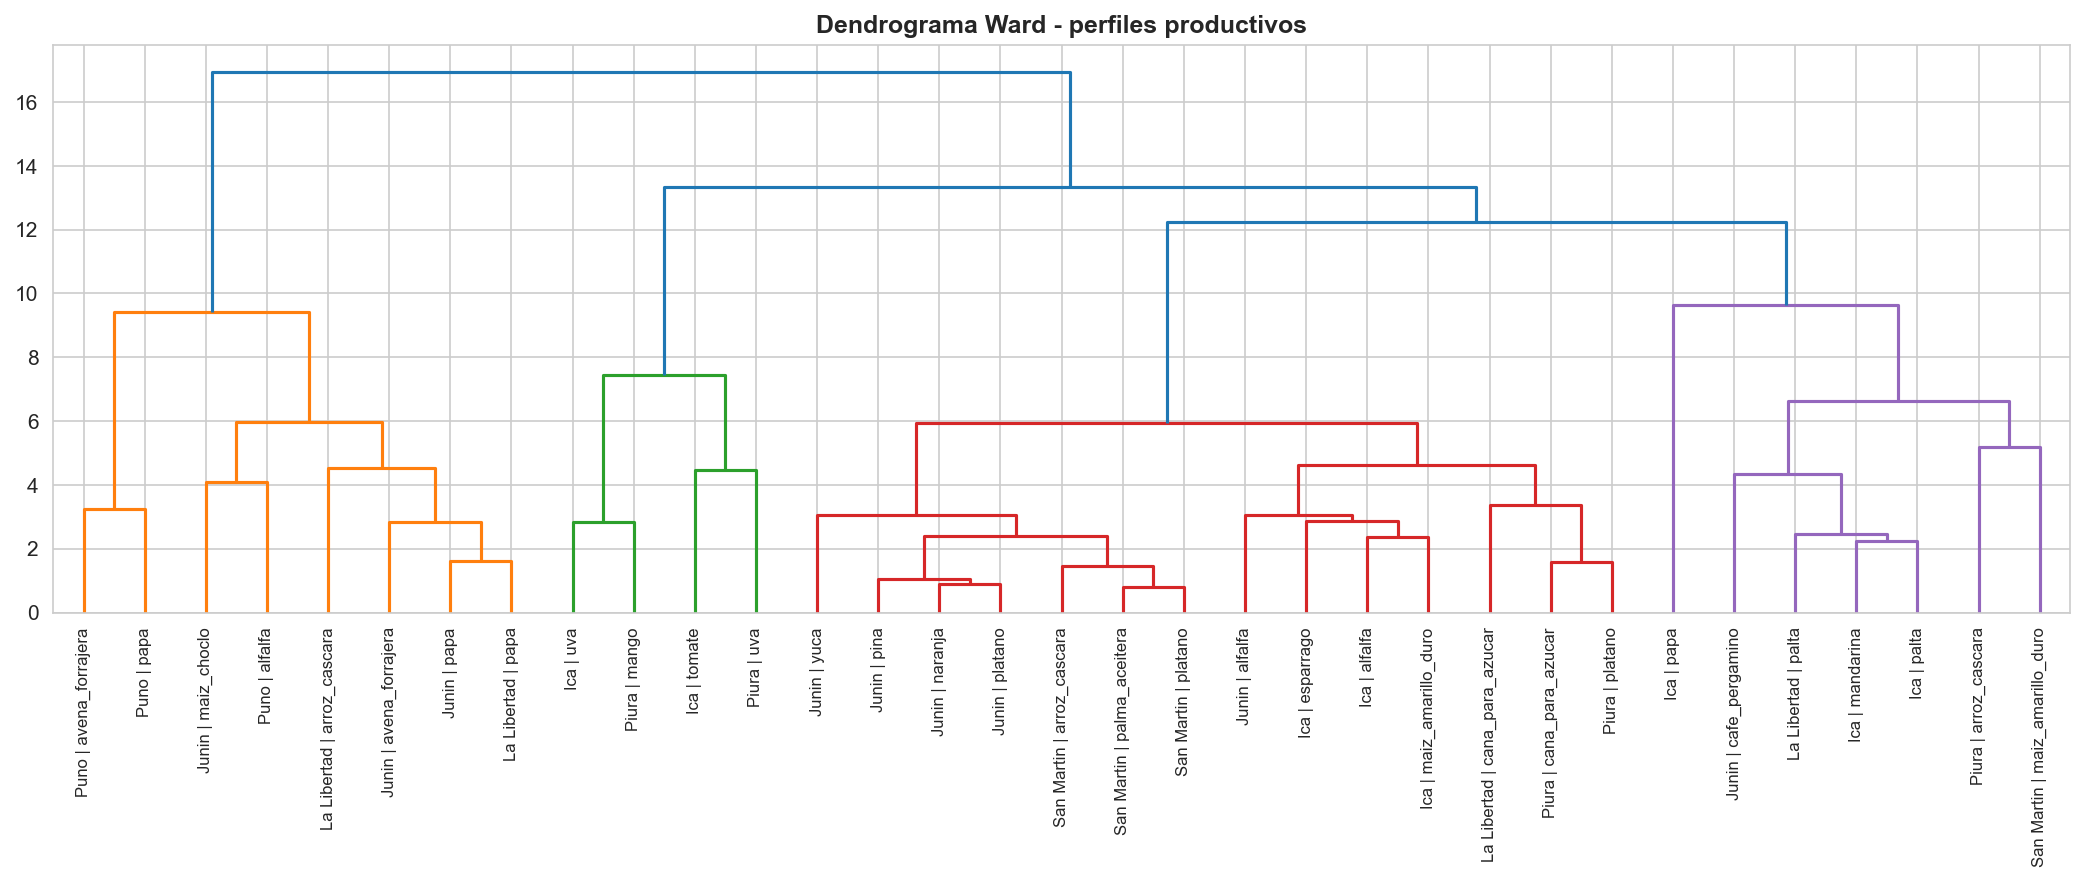
\includegraphics[width=0.48\textwidth]{06b_dendrograma_perfiles.png}
    \caption{Dendrograma Ward de los perfiles productivos. La línea roja marca la altura de corte que produce $K=6$ clusters.}
    \label{fig:dendro_b}
\end{figure}

\begin{figure}[h]
    \centering
    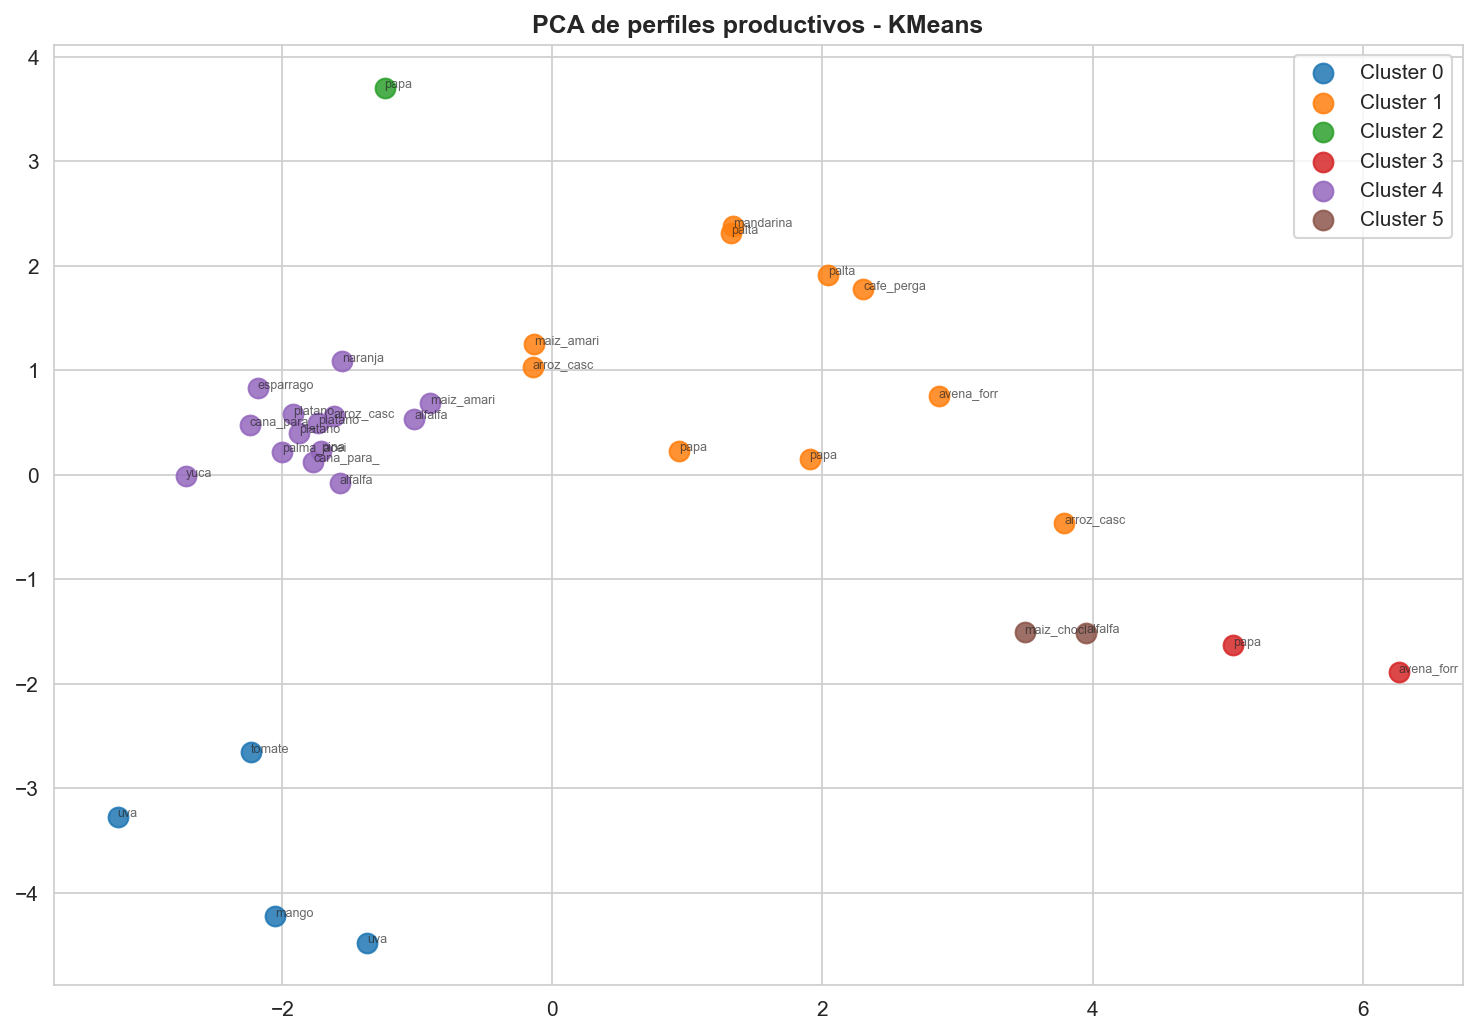
\includegraphics[width=0.46\textwidth]{06b_pca_perfiles.png}
    \caption{Proyección PCA de los perfiles productivos coloreada por cluster. La cercanía refleja similitud de calendario, no de región.}
    \label{fig:pca_b}
\end{figure}

\subsection{Validación: independencia de la geografía}
La prueba decisiva del modelo es su ARI con la región: 0.06, frente a 0.59 del enfoque convencional (Fig.~\ref{fig:comparativa}). El modelo propuesto ha roto el vínculo con la geografía. El ARI entre la partición convencional y la propuesta es de solo 0.18, confirmando que ambos modelos responden preguntas distintas: el convencional agrupa por territorio, el propuesto por comportamiento productivo. El menor Silhouette del modelo propuesto (0.30 vs.\ 0.51) no indica peor calidad, sino que resuelve un problema genuinamente más difícil en un espacio de \textit{features} donde no existe la redundancia geográfica que inflaba artificialmente la métrica del enfoque convencional.

\begin{figure}[h]
    \centering
    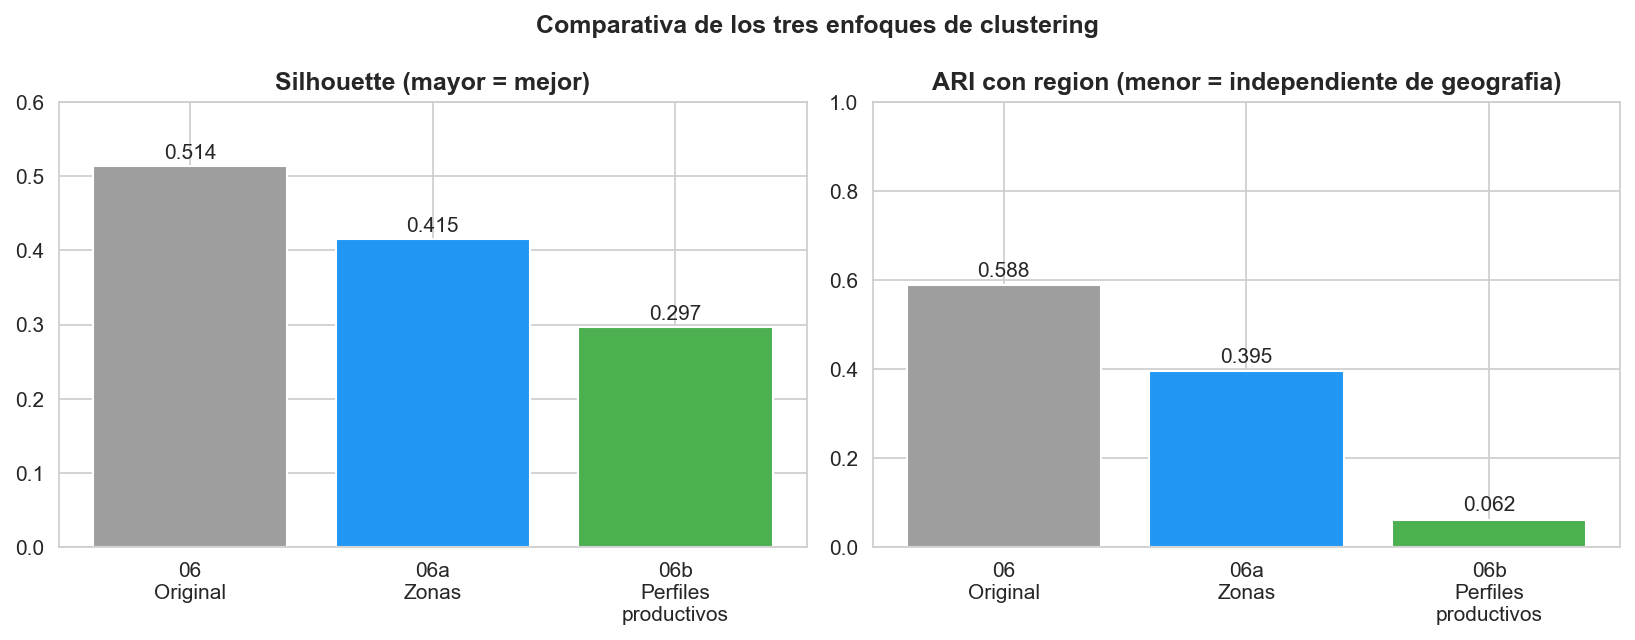
\includegraphics[width=0.48\textwidth]{comparativa_3enfoques.png}
    \caption{Comparación frente al enfoque convencional y a una variante territorial. El ARI con la región (derecha) confirma que solo el modelo de patrón productivo se independiza de la geografía.}
    \label{fig:comparativa}
\end{figure}

\section{Discusión y conclusiones}
Este trabajo propone y valida un modelo de \textit{clustering} que tipifica cultivos peruanos por su patrón productivo de forma independiente de la geografía. La contribución es doble. Metodológicamente, demostramos que el \textit{clustering} agroclimático convencional puede reproducir trivialmente la geografía cuando las \textit{features} climáticas están degeneradas, y que el Índice de Rand Ajustado frente a la región es un diagnóstico simple y efectivo que métricas internas como Silhouette no proporcionan. Aplicadamente, las seis tipologías de calendario productivo agrupan cultivos de regiones distintas que comparten estacionalidad, ofreciendo una base para la planificación de cosechas y la gestión del riesgo estacional --- por ejemplo, identificando qué cultivos concentran su oferta en los mismos meses pese a producirse en regiones alejadas.

Las limitaciones incluyen el número reducido de unidades (33 perfiles), que limita el poder estadístico y obliga a leer las tipologías como exploratorias; la asociación cultivo--distrito basada en criterio agronómico no validable directamente; y el uso de toneladas físicas en lugar de valor económico. Como trabajo futuro, el esquema de \textit{features} de estacionalidad puede enriquecerse con descriptores de tendencia interanual y combinarse con modelos predictivos por tipología para anticipar ventanas de cosecha. La conclusión principal es que tipificar el agro peruano exige separar explícitamente la dimensión territorial de la dimensión productiva: confundirlas conduce a modelos que solo redescubren el mapa.

\begin{thebibliography}{00}

\bibitem{bcrp2025} Banco Central de Reserva del Perú, ``Actividad económica: Enero 2025,'' Nota de Estudios 23-2025, Mar. 2025.

\bibitem{adex2026} Asociación de Exportadores (ADEX), ``Adex Hoy: Agroexportaciones 2025,'' Ed. 37081, Mar. 2026.

\bibitem{inia2019} H. Dorado, ``Uso de minería de datos en agricultura para hacer frente al cambio climático,'' INIA, 2019.

\bibitem{chapman2000} P. Chapman \textit{et al.}, ``CRISP-DM 1.0: Step-by-step data mining guide,'' SPSS Inc., 2000.

\bibitem{chapapria2024} L. Chapapría and C. Viladrich, ``Modelo predictivo agroclimático usando CRISP-DM,'' Alicia Concytec, 2024.

\bibitem{canchano2024} J. C. Canchano, ``Model for demand and price prediction of agricultural products using CRISP-DM,'' in \textit{Proc. IEEE Conf. Data Mining Applications}, 2024, pp. 1--6.

\bibitem{midagri2025} Ministerio de Desarrollo Agrario y Riego, ``Zonificación ecológica económica (ZEE),'' 2025.

\bibitem{una2023} Universidad Nacional del Altiplano, ``Propuesta de zonificación agroecológica para el desarrollo sostenible,'' Tesis, 2023.

\bibitem{midagrihist} Ministerio de Desarrollo Agrario y Riego, ``Series históricas de producción agrícola --- hoja c-18,'' 2025. [Online]. Available: \url{https://www.midagri.gob.pe/}

\bibitem{nasa2025} National Aeronautics and Space Administration, ``NASA POWER Data Access Viewer,'' 2025. [Online]. Available: \url{https://power.larc.nasa.gov/}

\end{thebibliography}

\end{document}
